% Chapter 3

\section{Derivational graph}\label{section:graph}
\lhead{Chapter 3. \emph{Derivational graph}}

\section{Introduction}
As we have seen in the previous chapter, existing approaches to Russian prefixation do not account for the full range of data. Moreover, they often do not agree on the data or some important data is missing and disregarded. This chapter is dedicated to describing a structure that allows to reach an agreement on the prefixation data and easily check the proposed generalizations, if a database, organized according to the definition provided here, is implemented. Material presented in this section is partially covered in \citet{ZinovaFilip:14b}.

After having discussed an efficient way of collecting and verifying the data, we will proceed to the discussion of the semantics of individual prefixes. This discussion has as a goal the formalization of prefix semantics that will allow us to build an account that predicts whether a particular verb containing certain prefixes exists and which aspect and semantics it has. I have shown that syntactic accounts, although organizing the initial mess of Russian prefixation, are not flexible enough to handle some cases. Such cases seam rear and exceptional at first, but upon careful examination they prove to be numerous and I believe they are important and point towards a finer organization of the whole system. That is why I propose to use the more flexible semantic framework to explain the workings of the prefixation system in Russian.

As has been noted by \citet{Tatevosov:09}, numerous works on semantics of prefixes \citep[][among others]{Avilova:64, Golovin:59, Lopatin:97, Tixonov:98} did not bring us closer to the understanding of the prefixation combinatorics. A new account by \citet{Kagan:book}, that is in spirit very close to what I propose here, also does not have the goal (and thus is not helpful for) the prediction of the possible combinations of verbal affixes. The crucial difference between the previous semantic accounts of Russian verbal prefixation and this work is the formalization of the semantics of prefixes, which will be provided in Chapter~\ref{Chapter6}. An important property of the formal part of the account is its capability to grasp by means of the semantic representation not only the semantics the prefix contributes to the derived verb, but also the semantic restrictions on its attachment. In section~\ref{section:semantics} I will prepare the ground for this formalization, providing informal descriptions of the semantics and attachment restrictions of individual prefixes after carefully investigating their properties. 

\subsection{Definitions}\label{section:chains:definition}
As we have seen in the previous chapter, some prefixed verbs can be derived in various ways. I propose to observe those possibilities carefully before excluding some of them that on the first sight do not fit neatly into the common model of verbal prefixation.

The notion of a `derivational chain' used here is inspired by \citet{Karcevski:27} who proposed that \textit{``[l]a valeur aspective d'un verbe d\'{e}pend de la place qu'il occupe dans la cha\^{i}ne de la d\'{e}rivation d\'{e}verbative''} [the aspectual value of a verb depends on its place in the chain of verbal derivation].

In the spirit of \citet{Karcevski:27}, the basic idea I pursue here is to infer the aspectual value (perfective or imperfective) of a given verb form from the derivational chain\footnote{In \citet{ZinovaFilip:14b} we call it \textit{derivational history}.} to , rather than from the pure syntactic structure, as it is done in contemporary syntactic analyses. I also want to put forward the idea that the derivational chain does not have to be unique for a given verb. To formalize \citeauthor{Karcevski:27}'s \citeyear{Karcevski:27} suggestions about the derivational chain, I propose the following definition:
\begin{definition}\label{def:history}
A verb V$_2$ is derived from a verb V$_1$ if and only if
\begin{enumerate}
\item both V$_1$ and V$_2$ are attested in the language;
\item there is a morphological operation (the extensive list of such operations is provided by \citealt{Shvedova:82}) such that it takes as an input the verb V$_1$ and provides as an output the verb V$_2$;
\item the meaning of V$_2$ can be monotonically (possibly not entirely compositionally) derived from the meaning of V$_1$;
\item there is no other verb V$_3$ such that V$_3$ is derived from V$_1$ and V$_2$ is derived from V$_3$.
\end{enumerate}
\end{definition}

To illustrate the above definition of a derivational chain, let us consider the verbs \textit{kupit'$^\PF$} and \textit{pokupat'$^\IPF$} `to buy.' There are three possible ways in which these verbs might be related, shown in \ref{chain:pokupat}.

\ex.\label{chain:pokupat}\ag.\label{chain:pokupat1}kup-i-t'$^\PF$ $\rightarrow$ *po-kup-i-t' $\rightarrow$ po-kup-a-t'$^\IPF$\\	
{to buy} $\rightarrow$ $\cdots$ $\rightarrow$ {to buy/to be buying}\\
\bg.\label{chain:pokupat2}kup-i-t'$^\PF$ $\rightarrow$ po-kup-a-t'$^\IPF$\\
{to buy} $\rightarrow$ {to buy/to be buying}\\
\bg.\label{chain:pokupat3}kup-i-t'$^\PF$ *$\rightarrow$ kup-a-t'$^\IPF$ *$\rightarrow$ po-kup-a-t'$^\IPF$\\
{to buy} *$\rightarrow$ {to bathe} *$\rightarrow$ {to buy/to be buying}\\

The derivation in \ref{chain:pokupat1} is excluded, because *\textit{pokupit'} does not exist (violation of the first condition). The derivation in \ref{chain:pokupat2} is fine with respect to the first and the second conditions and what we have to check for is the third condition. I.e., that there is no other verb such that it is derived from \textit{kupit'}$^\PF$ `to buy.'  A candidate verb, formally speaking, would be \textit{kupat'$^\IPF$}, but it has an unrelated meaning `to bathe someone' (violation of the second condition). This also means that \ref{chain:pokupat3} cannot be considered to constitute a derivational chain.  

As we have shown, the second chain, \ref{chain:pokupat2}, is a valid derivational chain, according to the three conditions above. However, it includes simultaneous (happening at one derivational step) attachment of two morphemes (the prefix \Prefix{po-} and the suffix \textit{-a-}), so it will not be discussed in this work. I will provide a computational account of verbal derivational morphology only for derivations including a single morpheme at each derivational step. I will not deal with those derivations that include a simultaneous addition of two morphemes (including cases of prefixation accompanied by the addition of the postfix) or discontinuous morphemes.

To provide an extension to this example, let us also consider the candidate derivational chains for the verb \textit{napokupat'} `to buy a lot,' presented in \ref{ex:napokupat}. The first candidate chain, \ref{ex:napokupat1}, demonstrates a violation of the third condition: there exists another verb (\textit{pokupat'} `to buy/be buying') such that it is derived from the verb \textit{kupit'} `to buy' and serves as a source verb for the derivation of the verb \textit{napokupat'} `to buy a lot.' So, despite the fact that the verb \textit{napokupat'} `to buy a lot' is (indirectly) derived from the verb \textit{kupit'} `to buy,' the derivation in \ref{ex:napokupat1} is not a valid derivational chain. On the other hand, the chain in \ref{ex:napokupat2} is a derivational chain, according to the definition above, although only the second step of it will receive an analysis in this work. 

\ex.\label{ex:napokupat}\ag.\label{ex:napokupat1}kup-i-t'$^\PF$ $\rightarrow$ na-po-kup-a-t'$^\PF$\\	
{to buy} $\rightarrow$ {to buy a lot}\\
\bg.\label{ex:napokupat2}kup-i-t'$^\PF$ $\rightarrow$ po-kup-a-t'$^\IPF$ $\rightarrow$ na-po-kup-a-t'$^\PF$\\
{to buy} $\rightarrow$ {to buy/to be buying} $\rightarrow$ {to buy a lot}\\

There is also another way to represent and store the information carried by the derivational chains, that is useful for computational purposes: a graph. Let us consider the following directed graph $D$: 
\begin{definition}\label{def:chain}
$D = (V,A)$, where V is a set of nodes labeled with verbs that are attested in the language and A is a set of ordered pairs of nodes. $\forall x,y \in V, (x,y) \in A$ iff 
\begin{enumerate}
\item $\llbracket y \rrbracket$ can be derived from $\llbracket x \rrbracket$
\item $~\nexists z \in V: (x,z) \in A \wedge (z,y) \in A$
\end{enumerate}
\end{definition}

In what follows, we will call such graph $D$ a \textit{derivational graph.} Paths in this graph are derivational chains that are defined by \ref{def:history}, whereby the first condition of the definition \ref{def:history} is subsumed by the definition of the set $S$, and the second and third condition in the definition of the derivational chain correspond to the first and the second conditions in the definition of the derivational graph, respectively.

In fact, a graph that is similar to the derivational graph described here, representing derivational relations between Russian verbs, exists: it is part of the OSLIN database (Open Source Lexical Information Network), described in \cite{Borik:12}.\footnote{Available online at \url{http://ru.oslin.org/index.php?action=aspect}} The problem with this graph is that it is far from being complete, as the lexical items included are taken from dictionaries and, as we have already discussed, this covers a relatively small amount of prefixed verbs and almost none of the multiply prefixed verbs.

Let me also mention another database of Russian prefixed verbs provided by the CLEAR (Cognitive Linguistics: Empirical Approaches to Russian) group at the University
of Troms{\o}.\footnote{available at \url{http://emptyprefixes.uit.no/}} According to the description on the website, ``[t]his database contains information on 1,981 imperfective verbs in Russian that form aspectual pairs via prefixation,'' aggregating entries from \citet{MAS,  Ozegov:01},  and \citet{Cubberly:82} that were approved by a panel of native speakers. This database, however, was constructed for the purpose of exploring the ``empty'' prefixes and thus is not a full derivational graph as it contains only verbs that form aspectual pairs (imperfective and perfective verbs with the same lexical meaning) via prefixation.

\subsection{Motivation}\label{section:chains:motivation}
Let me provide some motivation for the decisions made with respect to the (non) inclusion of the certain types of the potential edges in the graph. The notion of a derivation graph can be understood in different ways. For the broader picture, one may want to have a full graph with all possible connections. Such a graph will include edges connecting the nodes occupied by the verbs that are possibly semantically related but the relation is not evident for a native speaker. Another option is a graph with all the connections as long as the verbs are semantically connected. If no restriction on the complexity and the direction of morphological transitions is imposed, forms that are not directly derived from each other will be connected and the resulting structure will be a collection of ``nests,'' not ``chains.'' Such structure, for example, is discussed in \citealt{Janda:10}. A more restricted graph can also be useful: for example, a graph where only the most transparent relations are marked (those where semantic transitions are compositional). Another graph is extracted from the dictionary data by \citet{Janda:07a} for her analysis of the structure of aspectual clusters (for a restricted list of verbs). She lists not all the derived verbs but only one or two for each of the categories she distinguishes (Natural, Specialized, Complex Act, and Single Act Perfectives), thus reducing the complexity of the graph. In addition, the graph can be either directed or non-directed. 
 
The graph I propose to use is one with ``chain'' structures, which means that only direct connections are present and the nodes that can be reached through the transitive relations are not additionally directly connected. The second important point is that these chains will be later used to learn the rules of aspectual changes that happen at one derivational step. That is why it is good to include more relations, even those with not compositional semantic steps. On the other hand, it does not make sense to include those transitions where the semantic relation between the verbs is not transparent at all: as this is not a regular process, such verbs are listed in the dictionaries and do not allow for any generalization. 

I have decided to include also the derivations with simultaneous attachment of multiple affixes. They are not analyzed in this work, but among those derivations there are cases that must be taken into consideration in future work. For instance, it is claimed that some prefixes are attached simultaneously with postfixes. An example of such prefix is the cumulative \Prefix{na-}: if it is attached to the verb \textit{jest'} `to eat,' two verbs can be derived: \textit{najest'sja} `to eat until becoming full' and \textit{najest'} `to gain fat in some part of the body as the result of eating' (colloquial). The semantics of the first verb cannot be  monotonically derived from the semantics of the second one, as the component of gaining fat would have to be absent in the derived verb. So we have to accept that the verb \textit{najest'sja} `to eat until becoming full' is derived directly from the verb \textit{jest'} `to eat' by simultaneous attachment of the prefix and the postfix. Such verbs are not studied in this work, so I propose to include them in the derivational graph, but set them aside for the moment.
 
The derivational graph, built in accordance with definition~\ref{def:chain} would be a perfect starting point for the investigation of the individual prefixes, as one could use derivational chains for making generalizations about the verbal prefixes. For example, it would be easy to check whether a certain prefix allows a subsequent imperfectivization or can be attached on top of the other prefix: one only would have to check the properties of the verbs that are connected with the edges in the derivational graph. 

Consider the verb {\it pisat'} `to write' and the verb {\it dopisyvat'} `to finish writing.' There is only one possible path from the verb {\it pisat'} `to write' to the verb {\it dopisyvat'} `to finish writing', in the derivational graph fragment illustrated by figure~\ref{tree:dopisyvat}. This path is written as a derivational chain under \ref{deriv1-1}. Although the nodes for another way, shown in \ref{deriv1-2}, are present in the derivational graph, one of the edges (between the verb \textit{pisyvat'} `to write occasionally' and the verb \textit{dopisyvat'} `to finish/be finishing writing') is missing because of the semantic restriction (second condition in \ref{def:history} or first condition in \ref{def:chain}).

\ex.\label{deriv1} \ag.\label{deriv1-1}pisat'$^\IPF$ $\rightarrow$ dopisat'$^\PF$ $\rightarrow$ dopisyvat'$^\IPF$\\
{to write} $\rightarrow$ {to finish writing} $\rightarrow$ {to finish/be finishing writing}\\
\bg.\label{deriv1-2}pisat'$^\IPF$ $\rightarrow$ pisyvat'$^\IPF$ $\nrightarrow$ dopisyvat'\\
{to write} $\rightarrow$ {to write occasionally} $\rightarrow$ {to finish/be finishing writing}\\

\begin{figure}
\begin{center}
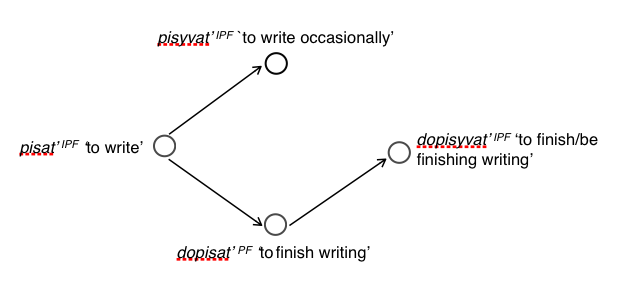
\includegraphics[scale=0.6]{treedopisyvat.png}
\caption{A fragment of the derivational tree including the verb \textit{pisat'} `to write'\label{tree:dopisyvat}}
\end{center}
\end{figure}

The fragment of the derivational graph, presented in \ref{tree:dopisyvat}, provides evidence for the hypothesis that if a verb contains both the prefix \Prefix{do-} and the imperfective suffix, it is imperfective. However, this hypothesis is quickly rejected on the basis of the other part of the graph: if one searches through the paths from the verb {\it pisat'} `to write' to the verb {\it dozapisyvat'} `to finish/be finishing writing down/recording,' one finds two different derivational chains in the derivational graph, as shown in \ref{tree:dozapisyvat}. The first derivational chain, linearized in \ref{deriv:dozapisyvat1}, provides evidence against the proposed hypothesis, as the verb in the end of this chain is perfective and contains both the imperfective suffix and the prefix \Prefix{do-}. 

\ex.\label{deriv:dozapisyvat}\ag.\label{deriv:dozapisyvat1}pisat'$^\IPF$ $\rightarrow$ zapisat'$^\PF$ $\rightarrow$ zapisyvat'$^\PF$ $\rightarrow$ dozapisyvat'$^\PF$\\
{to write} $\rightarrow$ {to record} $\rightarrow$ {to (be) record(ing)} $\rightarrow$ {to finish recording}\\
\bg.\label{deriv:dozapisyvat2}pisat'$^\IPF$ $\rightarrow$ zapisat'$^\PF$ $\rightarrow$ dozapisat'$^\PF$ $\rightarrow$ dozapisyvat'$^\IPF$\\
{to write} $\rightarrow$ {to record} $\rightarrow$ {to finish recording} $\rightarrow$ {to (be) finish(ing) recording}\\				

\begin{figure}
\begin{center}
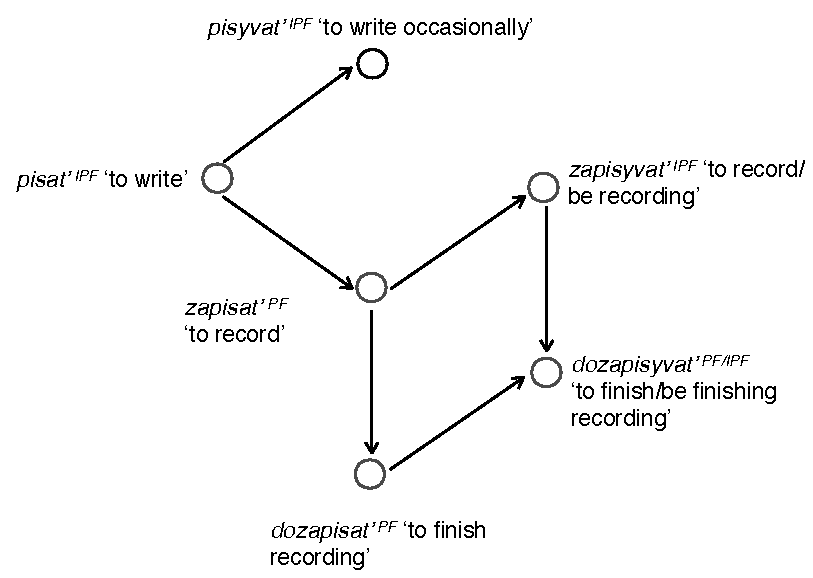
\includegraphics[scale=0.7]{treedozapisyvat.pdf}
\caption{A fragment of the derivational tree including the verb \textit{pisat'} `to write' and \textit{dozapisyvat'} `to (be) finish(ing) recording'\label{tree:dozapisyvat}}
\end{center}
\end{figure}			

The example above is just one illustration of how the derivational graph defined in \ref{def:chain} can be used to check possible generalizations about the properties of Russian prefixed verbs. Such a graph, however, does not exist in the form of a human-created resource\footnote{The graph itself exists by definition, so what I mean here is some resource that stores this graph and allows to extract information from it.} and some doubt even the possibility of writing it down in an overt form. For example, \citet[625]{Janda:07a} writes that ``exhaustive listings of verbs would be unwieldy, and, given the ad-hoc open-class nature of Specialized Perfectives and Complex Acts, such lists could never be definitive.'' \citet[626]{Janda:07a} also regards most of those verbs that are not listed in the dictionaries and constructed spontaneously by the speakers to be not the core part of the verbal cluster. 

I do not agree with the marginal status of such verbs and consider them an important part of the Russian verbal system. Moreover, I claim that there is a way to construct a derivational graph described here. To do this, I propose to take the following approach: I will base the generalizations in this chapter on the data about parts of this graph that are built using introspection and corpora/search engines data. Afterwards I will propose a formal account that is capable of predicting which vertices and edges, apart from those already included on the basis of the dictionary data, should be included in the derivational graph (at the moment only with respect to five prefixes I analyze in this work). I will then check those predictions at least partially against corpora and search engine data. The output of the computational system can be then used to build a larger part of the derivational graph on the basis of the dictionary data or OSLIN database.

\subsection{Predicting the aspect of the derived verb}
The property that drives the analysis proposed here and is implicitely rejected by the syntactic theories of Russian prefixation, as we have discussed in section~\ref{subsection:bi:predictions}, is that a given verb does not need to have a unique derivational history. For example, the biaspectual verb \textit{dozapisyvat'} `to (be) finish(ing) recording/writing down' is associated with two derivational chains given in \ref{deriv:dozapisyvat}, whereby one of them motivates the perfective aspect of the whole verb \ref{deriv:dozapisyvat1}, while the other motivates the imperfective aspect of the same verb \ref{deriv:dozapisyvat2}.

For a verb having two derivational chains implies that it may be ambiguous with respect to grammatical aspect: each derivational chain yields exactly one grammatical aspect for the derived verb, either perfective or imperfective. The context then presumably selects one of the derivational chains, and consequently, either the perfective or imperfective aspect of the verb, contrary to the syntactic approaches (in their existing form), which can only provide one derivational chain for any given complex verb form due to formal restrictions on the positions of different affixes.

This is desirable given that, judging from the data, the verb \textit{dozapisyvat'} `to (be) finish(ing) recording/writing down' is genuinely ambiguous with respect to the perfective/imperfective distinction, and it is the context that enforces one or the other grammatical aspect assignment. Note that the two derivational chains in \ref{deriv:dozapisyvat1} and \ref{deriv:dozapisyvat2} straightforwardly follow from the two general patterns that are widely accepted as governing the formation of Russian verbs, although there are also some exceptions to them that we have discussed in section~\ref{section:new:perfectivity}:

\begin{enumerate}
\item the output of a prefixation is perfective;   
\item adding the imperfective suffix to a verb yields an imperfective verb. 
\end{enumerate}

The root verb in \ref{deriv:dozapisyvat1} and \ref{deriv:dozapisyvat2} is the primary imperfective verb \textit{pisat'} `to write/to be writing.' Adding the prefix \textit{za}- to it yields a perfective verb, in compliance with (1), and the addition of the imperfective suffix -\textit{yva}- yields a secondary imperfective verb, following (2), which in turn serves as the basis for the prefixation with the completive prefix \Prefix{do-}. The result is the perfective verb \textit{dozapisyvat'} `to finish recording/writing down,' in compliance with (1).  In \ref{deriv:dozapisyvat2}, the second and the third steps are reversed, leading to the imperfective category assignment to the derived verb \textit{dozapisyvat'} `to finish/be finishing recording/writing down.'

Just as in the syntactic accounts (discussed in~\ref{section:old:prefixes}), it is the final step of the derivation that determines the aspect of the whole complex verb. Together with the assumption that each prefix (including the usage) occupies a fixed position in the syntactic tree this leads to the prediction that structural properties of the verbs that have the same outermost prefixes are always the same. For example, the verbs that we have just considered, \textit{dopisyvat'}$^\IPF$ `to (be) finish(ing) writing' and \textit{dozapisyvat'}$^{\IPF/\PF}$ `to finish/be finishing recording/writing down,' are either both perfective or both imperfective on any existing syntactic prefixation account, as they contain the same outermost prefix \Prefix{do-} and its position in the tree determines the aspect of the whole verb. On the account advocated here, there is an evident difference between those verbs, as the order of the derivational steps is determined based on all possible derivational chains that are constructed in compliance with the definition~\ref{def:history}. While the verb \textit{dozapisyvat'}$^{\IPF/\PF}$ `to (be) finish(ing) writing down/recording' has two derivational chains, as has been shown by \ref{deriv:dozapisyvat1} and \ref{deriv:dozapisyvat2}, which motivates its biaspectual nature, the imperfective verb \textit{dopisyvat'}$^\IPF$ `to finish/be finishing writing' has only one, as has been shown by \ref{deriv1}.

Another example, that we have already mentioned in \ref{subsection:bi:apply}, is the verb \textit{dovy\v{s}ivat'} `to finish embroidering'. It contains the same type of affixes as \textit{dozapisyvat'} `to finish recording/writing down' in \ref{deriv:dozapisyvat}. Namely, a completive prefix \Prefix{do-}, one more prefix commonly characterized as a lexical prefix, and the imperfective suffix. The verbs \textit{dovy\v{s}ivat'} `to finish embroidering' and \textit{dozapisyvat'} `to finish recording/writing down' are morphologically alike and thus there is no structural difference between them on any existing syntactic account of Russian verbal prefixation, as the structure of the verb and the order of the affix attachment is determined only on the basis of the syntactic properties of the affixes.
 
It turns out that these verbs are clearly different for most native speakers: while the perfective uses of the verb \textit{dozapisyvat'} `to finish recording/writing down' are judged odd by some speakers (as claimed by Sergei Tatevosov, personal communication), all the native speakers that I consulted agree that the verb \textit{dovy\v{s}ivat'} `to finish embroidering' can be used as a perfective verb. Moreover, most of those speakers are very reluctant to accept \textit{dovy\v{s}ivat'} `to finish embroidering' as an imperfective verb. At the same time, they reject the existence of the verb $^?$\textit{dovy\v{s}it'}$^\PF$ `to finish embroidering.' This behavior is easily explained by means of the relevant part of the derivational graph, presented in Figure~\ref{tree:dovyshivat}. For the group of speakers who reject the existence of the verb $^?$\textit{dovy\v{s}it'}$^\PF$ `to finish embroidering', the derivation in \ref{deriv:dovyshivat2} is not available, as it requires the verb $^?$\textit{dovy\v{s}it'}$^\PF$ `to finish embroidering' to be attested. Thus the verb \textit{dovy\v{s}ivat'} `to finish embroidering' cannot be assigned the imperfective aspect.

\ex.\label{deriv:dovyshivat}\ag.\label{deriv:dovyshivat1}\v{s}it'$^\IPF$ $\rightarrow$ vy-\v{s}it'$^\PF$ $\rightarrow$ vy-\v{s}-iva-t'$^\IPF$ $\rightarrow$ do-vy-\v{s}-iva-t'$^\PF$\\
{to sew} $\rightarrow$ {to embroider} $\rightarrow$ {to embroider/be embroidering} $\rightarrow$ {to finish embroidering}\\
\bg.\label{deriv:dovyshivat2}\v{s}it'$^\IPF$ $\rightarrow$ vy-\v{s}it'$^\PF$ $\rightarrow$ do-vy-\v{s}it'$^\PF$ $\rightarrow$ do-vy-\v{s}-iva-t'$^\IPF$\\
{to sew} $\rightarrow$ {to embroider} $\rightarrow$ {to finish embroidering} $\rightarrow$ {to finish/be finishing embroidering}\\

\begin{figure}
\begin{center}
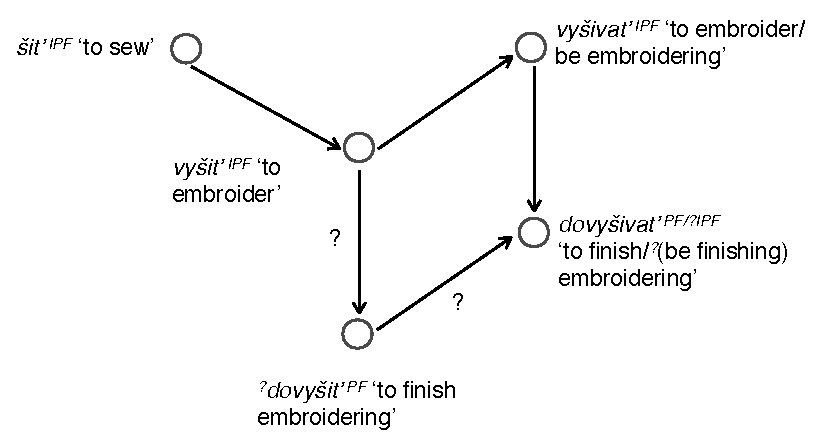
\includegraphics[scale=0.7]{treedovyshivat.pdf}
\caption{A fragment of the derivational tree including the verb \textit{\v{s}it'} `to sew' and \textit{dovy\v{s}ivat'} `to finish embroidering'\label{tree:dovyshivat}}
\end{center}
\end{figure}		

Another question to ask is whether there are prefixes such that the result of the prefixation with them is always a perfective verb, i.e., whenever a verb contains such a prefix, all derivational chains will have prefixation as the last derivational step. Although this is one of the classical characteristics of the superlexical prefixes \citep[see, e.g.][]{Ramchand:04, Svenonius:04a, Romanova:06}, \citet{Tatevosov:07, Tatevosov:09} provides numerous counterexamples to such constraint. In the account proposed in \citealt{Tatevosov:09}, the constraints are formulated in different terms: either the prefixes must be attached before the imperfective suffix or to a formally imperfective verb. Only the distributive prefix \textit{po}- that, according to \citet{Tatevosov:09}, occupies the left periphery of the verb, is then clearly a prefix of such a type that the verb that contains it is necessarily perfective. We will further investigate the ability of individual prefixes discussed here to constitute a part of an imperfective verb.
